\section{Results}
\label{sec:04-results}

\subsection{Qualitative results}

To show the results of global motion estimation it is easier to use some qualitative information, also because the reader will understand it straightforwardly.

One of the applications that shows intuitively the implications of global motion estimation is camera motion compensation. 
Basically, if the video is recorded by a camera which is moving, we will see the two types of motion explained in \cref{sec:01-intro}: apparent and real. The aim of camera-motion compensation is to detect and remove the (apparent) motion which is caused only by the (ego)motion of the camera.

To show the results obtained we reported in image \cref{fig:qualitative-results} an example in which the reader can observe:
\begin{itemize}
    \item the previous frame in \cref{fig:prev-frame};
    \item the next frame in \cref{fig:curr-frame};
    \item the compensated frame, obtained by compensating camera motion in the previous frame, in \cref{fig:compensated};
    \item the absolute difference between next and previous frame in \cref{fig:diff-curr-prev}, which gives an idea of how strong is the motion in which parts of the image;
    \item the motion field generated by the camera as returned by our estimation procedure in \cref{fig:est-mf};
    \item the absolute difference between the next frame and the compensated one in \cref{fig:diff-curr-comp}.
\end{itemize}

\begin{figure*}[htbp]

    \begin{subfigure}[b]{0.3\textwidth}
        \centering
        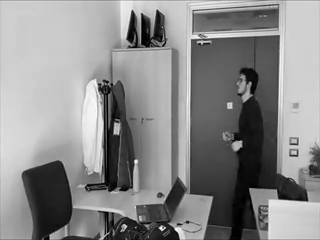
\includegraphics[width=1\textwidth]{../assets/images/04-prev-frame.png}
        \caption{Previous frame.}
        \label{fig:prev-frame}
    \end{subfigure}
    \hfill
    \begin{subfigure}[b]{0.3\textwidth}
        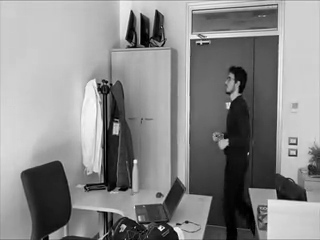
\includegraphics[width=1\textwidth]{../assets/images/04-curr-frame.png}
        \caption{Next frame.}
        \label{fig:curr-frame}
    \end{subfigure}
    \hfill
    \begin{subfigure}[b]{0.3\textwidth}
        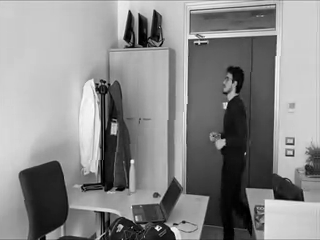
\includegraphics[width=1\textwidth]{../assets/images/04-compensated.png}
        \caption{Compensated previous frame.}
        \label{fig:compensated}
    \end{subfigure}
    
    \vspace{0.5em}

    \begin{subfigure}[b]{0.3\textwidth}
        \centering
        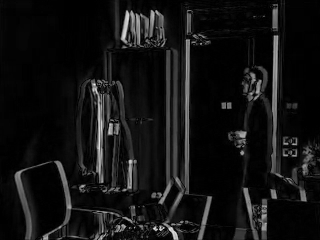
\includegraphics[width=1\textwidth]{../assets/images/04-diff-curr-prev-1.png}
        \caption{Absolute difference between current and previous frame (white areas are where we detect motion).}
        \label{fig:diff-curr-prev}
    \end{subfigure}
    \hfill
    \begin{subfigure}[b]{0.3\textwidth}
        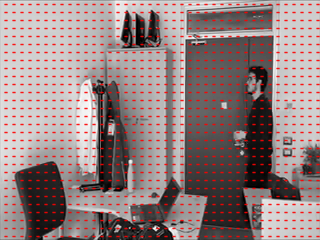
\includegraphics[width=1\textwidth]{../assets//images/04-camera-motion-1.png}
        \caption{Global motion field estimated by our procedure, it corresponds to the motion generated by the camera.}
        \label{fig:est-mf}
    \end{subfigure}
    \hfill
    \begin{subfigure}[b]{0.3\textwidth}
        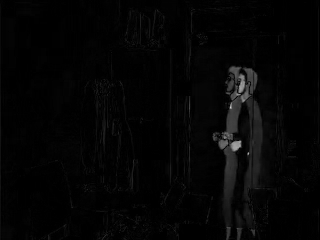
\includegraphics[width=1\textwidth]{../assets/images/04-diff-curr-comp.png}
        \caption{Absolute difference between current and compensated frame, the only object in white is the only actually moving.}
        \label{fig:diff-curr-comp}
    \end{subfigure}

    \caption{Qualitative results.}
    \label{fig:qualitative-results}
\end{figure*}

\paragraph{How to interpret qualitative results} We should be able to notice in the results that the motion that we detect between the two frames (previous and next) is pretty large. In fact, by using the absolute difference between frames, we can see that a big part of the visual field seems to be moving in \cref{fig:diff-curr-prev}.

However, by computing the motion generated by the camera egomotion, we find out that most of the shift we register is apparent.
By estimating the motion generated by the camera, which is reported in  \cref{fig:est-mf}, we can compensate the apparent motion in the previous frame.
When we compensate the previous frame we \textit{remove} all the motion due to apparent motion and, therefore, if we compare the current frame and the compensated frame (see \cref{fig:diff-curr-comp}) we are able to isolate real motion.

The results shown are consistent since the video from which the frames are taken was recorded with the camera moving in the horizontal direction while the person in the video was walking.

\subsection{Quantitative results}

To perform a numeric quantitative analysis of the results produced by the algorithm we used, once again, the compensation of the previous frame. Basically, in a video sequence where there is no real motion, but only camera motion, the compensation of the apparent motion should be enough tho make the current and the compensated frame identical.

Therefore, in \cref{tab:psnr}, we present some PSNR values for different video sequences. We annotated the table with some considerations about the videos, since PSNR value is influenced also about properties of the video like the strength of motion or the presence/absence of real motion.

For instance, in the case where there are medium or big objects, like the last two entries of the table, the PSNR turns out to be low, since the model isn't able to distinguish between object and camera motion.

Better results can be observed in the first two entries of the table, where the moving object are considerably smaller w.r.t. the background, and the background presents some complex pattern, which enables the algorithm to better detect its motion.

\begin{table}
    \label{tab:psnr}
    \begin{tabular}{ll|rrrr}
    \toprule
    Video & Properties & Average & Variance & Maximum & Minimum \\
    \midrule
    {\small\texttt{pan240.mp4}} & {\small Fast motion} & \(22.724\)  & \(5.125\)  & \(27.802\) & \(17.981\)  \\

    {\small\texttt{coastguard\_qcif.mp4}} & 
        \begin{tabular}{@{}c@{}}{\small Two objects moving,}\\{\small background moving}\end{tabular}
    & \(22.733\)  & \(2.194\)  & \(26.875\) & \(15.158\)  \\
    
    {\small\texttt{foreman.mp4}} & 
        \begin{tabular}{@{}c@{}}{\small Big object moving,}\\{\small still background}\end{tabular}
        & \(19.677\)  & \(18.443\)  & \(30.436\) & \(11.746\)  \\
        
    {\small\texttt{numeri\_del\_piero.mp4}} & 
        \begin{tabular}{@{}c@{}}{\small Medium object moving,}\\{\small moving background}\end{tabular}
    & \(19.072\)  & \(13.642\)  & \(47.722\) & \(16.323\)  \\
    

    \bottomrule
\end{tabular}
    \caption{PSNR results on some video samples}
\end{table}    
